
\documentclass[12pt]{article}
\usepackage{geometry} % see geometry.pdf on how to lay out the page. There's lots.
\geometry{a4paper} % or letter or a5paper or ... et
\usepackage{graphicx}
\usepackage{float}
% \geometry{landscape} % rotated page geometry

% See the ``Article customise'' template for come common customisations

\title{CmpE 462 Homework 3}
\author{Alptekin Orbay \\ 2015400252}

%%% BEGIN DOCUMENT
\begin{document}

\maketitle

	The dataset is divided as 350 instances for training set and 50 instances test set. The decision is made empirically. 350 instances are good candidate for representing the general data distribution. Data has some critical features and some joined class areas. This configuration is chosen from tests from  300-360 training set configurations.
	The output is posterior probabilities of instances for each classes which are three real numbers between 0 and 1. The aim is to make the posterior probability closes to 1 for $i^{th}$ output of a instances that belongs to the  $i^{th}$class. In shot, three real number between 0 and 1 that illustrates posterior probability that shows the belonging probability of an instances to the class. For classification, the maximum posterior probability of the outputs determine the class. For example, for class 1-2-3, a output [0.1 0.1 0.8] shows that the instances belongs to the $3^th$ class. Furthermore, the error function is cross entropy that is $\sum_i{- r_i\log (p_i)}$.
$r_i$ is the real value of the instances such that a class 2 instance has $ r_1 = 0 , r_2 = 1, r_3 = 0$  
values.

\begin{figure}[H]
\begin{center}
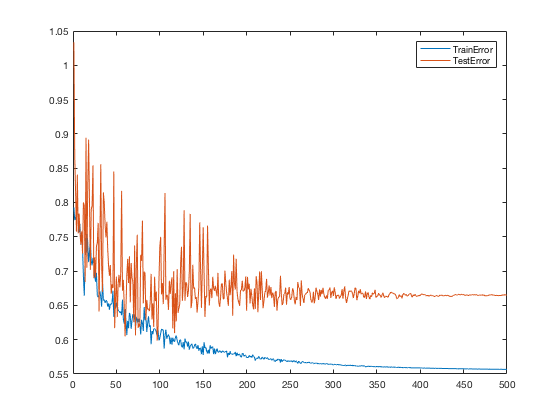
\includegraphics[scale=0.5]{images/train_test_error}
\caption{Test and Train Error}
\label{default}
\end{center}
\end{figure}
\begin{figure}[H]
\begin{center}
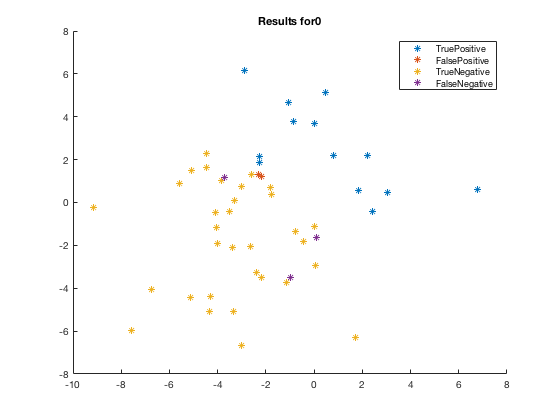
\includegraphics[scale=0.5]{images/class0}
\caption{TP TN FN FP for Class 0}
\label{default}
\end{center}
\end{figure}
\begin{figure}[H]
\begin{center}
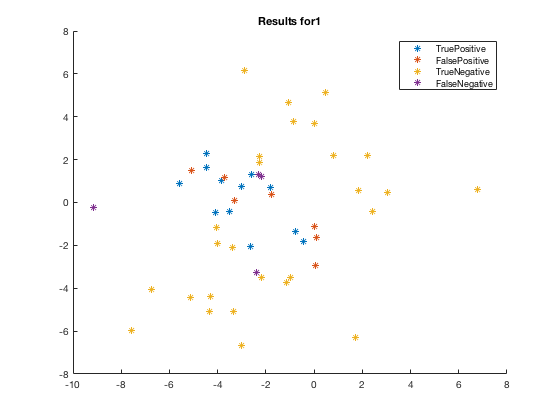
\includegraphics[scale=0.5]{images/class1}
\caption{TP TN FN FP for Class 1}
\label{default}
\end{center}
\end{figure}
\begin{figure}[H]
\begin{center}
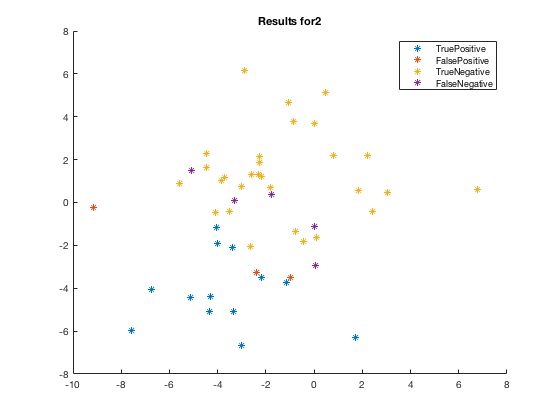
\includegraphics[scale=0.5]{images/class2}
\caption{TP TN FN FP for Class 2}
\label{default}
\end{center}
\end{figure}

\begin{figure}[H]
\begin{center}
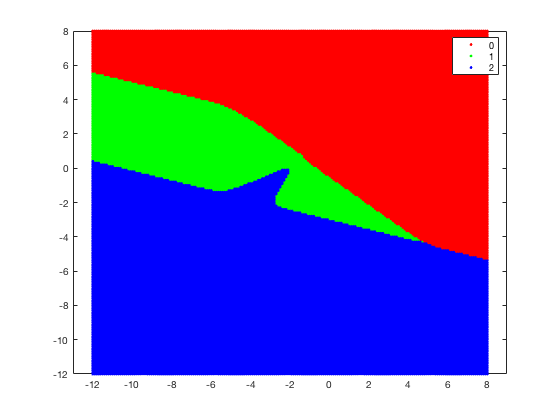
\includegraphics[scale=0.5]{images/boundary}
\caption{Decision Boundaries}
\label{default}
\end{center}
\end{figure}


\end{document}